\chapter{Teoremas de conservación para el caso de una partícula}	
\chaptermark{Teoremas de conservación}


\section{Conservación de la energía mecánica}

Supongamos un partícula sometida a la acción de un campo de fuerzas $\vec F$.

$\left. \begin{array}{ll}
\vec F\cdot \dd \vec r =W = \dd \mathcal E_c\\
\vec F\cdot \dd \vec r= - \dd \mathcal E_p \; (*)\end{array} \right\}
\qquad \boldsymbol{\dd \subrayado{\mathcal E_c=-\dd \mathcal E_p}}$

\begin{multicols}{2}
Siempre que $\vec F$ sea un \emph{\colorbox{LightYellow}{campo conservativo}}.

Si $\dd \mathcal E_c=-\dd \mathcal E_p \to \dd \mathcal E_c+\dd \mathcal E_p=0 \to \dd (\mathcal E_c +\mathcal E_p)=0 \Rightarrow$

\begin{equation}
\label{conserva-E}
	\subrayado{\boxed{\;\boldsymbol{ \mathcal Ec +\mathcal E_p=cte }\;}} 
\end{equation}
en campos conservativos.
\begin{figure}[H]
	\centering
	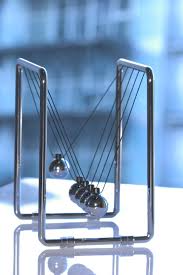
\includegraphics[width=0.2\textwidth]{imagenes/imagenes04/T04IM01.png}
	\caption*{Cuna de Newton}
\end{figure}
\end{multicols}


Se llama \emph{energía mecánica} a la suma de las energías cinética y potencial $\to$ en presencia de campos conservativos, la energía mecánica es constante, se conserva.

$$\boxed{\;\mathcal E_{c_1} +\mathcal E_{p_1}=\mathcal E_{c_2} +\mathcal E_{p_2}\;} \qquad \text{(en campos conservativos)} $$


\section{Conservación de la cantidad de movimiento.}

\begin{multicols}{2}
$\displaystyle \vec F=\dv{\vec p}{t}$, 

en el caso en que $\vec F=\vec 0$,
\begin{equation}
\label{conserva-p}
\subrayado{\boxed{ \;\boldsymbol{ \overrightarrow{ p} = \overrightarrow{cte}}\;} \qquad \text{ (si } \vec F=\vec 0	)}
\end{equation}
\\
\begin{figure}[H]
	\centering
	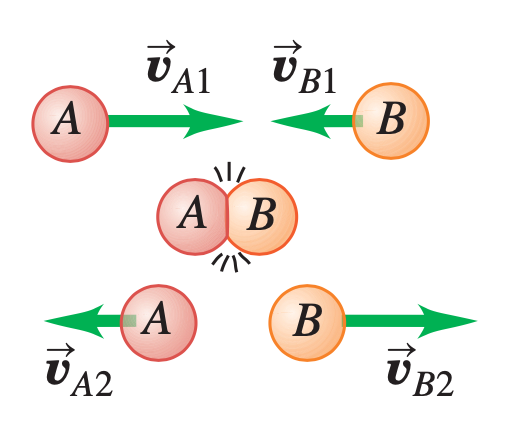
\includegraphics[width=0.3\textwidth]{imagenes/imagenes04/T04IM02.png}
	\caption*{Choque elástico}
\end{figure}
\end{multicols}

\section[Momento angular. Conservación del momento angular]{Momento angular. Conservación del momento angular\sectionmark{Conservación del momento angular}}
\sectionmark{Conservación del momento angular}

\begin{multicols}{2}
El momento angular o momento cinético es una magnitud física que representa la cantidad de movimiento de rotación de un objeto. Desempeña, en rotaciones, un papel análogo al momento lineal en las traslaciones. Sus unidades en el $SI$ son $\ \mathrm{kg\ m\ s}^{-1}$
\begin{figure}[H]
	\centering
	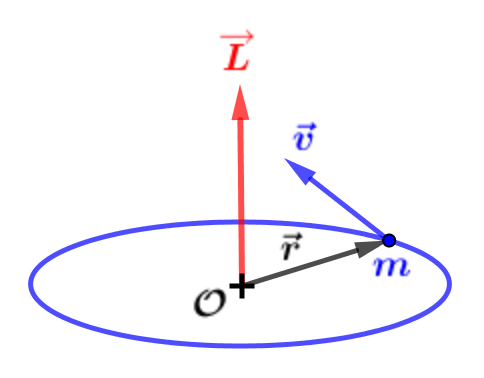
\includegraphics[width=0.4\textwidth]{imagenes/imagenes04/T04IM03.png}
\end{figure}
\end{multicols}

\colorbox{LightYellow}{Momento angular} respecto de un punto $\mathcal O$: 
$\quad \boldsymbol{ \subrayado{ \overrightarrow{L}=\vec r \times \vec p } } \quad$ es perpendicular al plano $\{\vec r  ,  \vec p\}$.

$\vec L=\vec r \times \vec p$
$\qquad \vec L \bot \vec r;\quad \vec L \bot \vec p$

Si la partícula considerada se mueve en un plano, la dirección de $\vec L$ permanecerá invariante ($\bot \vec r;\ \bot \vec v; \ \bot \text{ plano } \{ \vec r,\vec v \}$), con $\vec v \bot \vec r$ y $v=\omega r \ \to \ L=mrv \sin 90^o=mrw=mr^2 \omega $

$\vec L \ \parallel \ \vec \omega \ \Rightarrow \  \boldsymbol{\vec L =mr^2 \vec \omega}$
\begin{figure}[H]
	\centering
	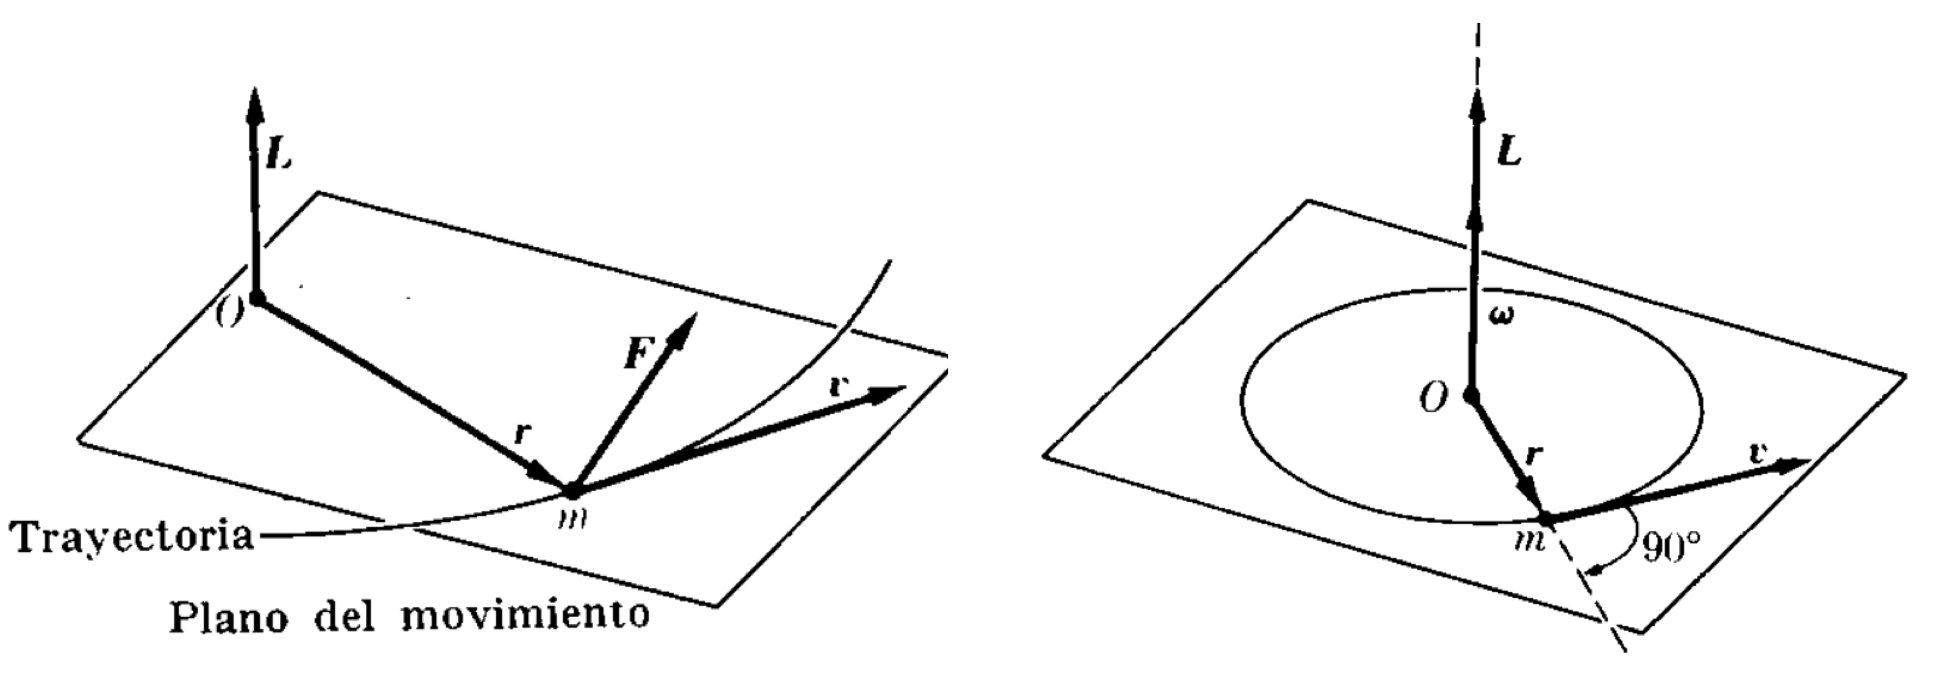
\includegraphics[width=1\textwidth]{imagenes/imagenes04/T04IM18.png}
\end{figure}

Si el movimiento en el plano no es circular sino curvilíneo, usaremos las componentes polares del vector velocidad (ver sección \ref{veloc-polares}).

\begin{multicols}{2}
	$\vec v=\vec v_r+\vec v_\theta \to \vec L=m\vec r \times (\vec v_r+\vec v_\theta)=m\vec r \times \vec v_\theta$ 
\textcolor{gris}{$\quad \vec r \times \vec v_r=\vec 0, \text{ paralelos}$}

Por definición, $\vec v_{\theta} \bot \vec r$, luego, en módulo:

$L=mrv_\theta \sin 90^o = mrv_\theta$. 

Como $\displaystyle v_\theta =r \dv{\theta}{t}  \to L=m r^2 \dv{\theta}{t}$
\begin{figure}[H]
	\centering
	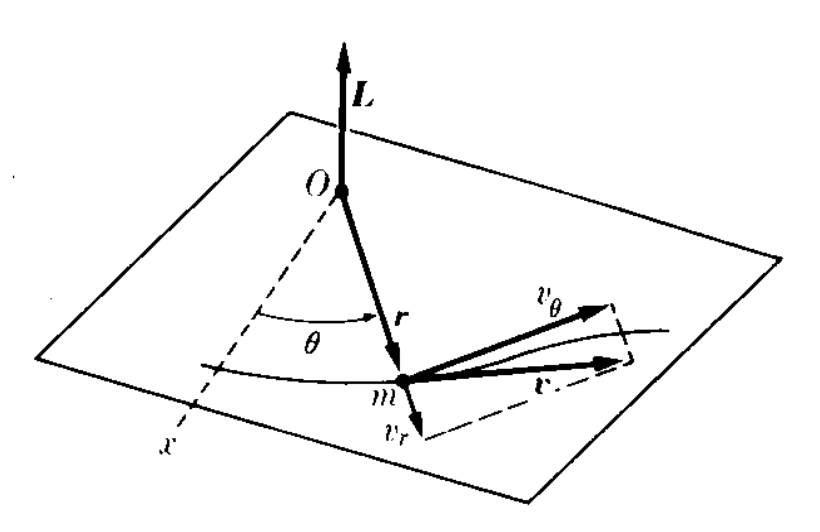
\includegraphics[width=.5\textwidth]{imagenes/imagenes04/T04IM19.png}
\end{figure}	
\end{multicols}

$\vec L=\vec r \times \vec p=
\left| \begin{matrix}
 \vec i&\vec j&\vec k \\ x&y&z \\ p_x&p_y&p_z
\end{matrix} \right| $

Si el movimiento es en el plano $XY$, $\ z=0,\ p_z=0 \to L_x=L_y=0$. Solo queda componente $L_z$: 
\emph{\textbf{\colorbox{LightYellow}{el momento angular es perpendicular}}} 
\emph{\textbf{\colorbox{LightYellow}{al plano de movimiento}}} 
$XY$.

Derivando respecto del tiempo: $\displaystyle \ \dv{\vec L}{t}=\dv{\vec r}{t}\times \vec p + \vec r \times \dv{\vec p}{t}$

$\displaystyle \vec v \; ||\; \vec p  \to \dv{\vec r}{t} \times \vec p=\vec v \times \vec p = \vec 0; \qquad \dv{\vec p}{t}=\vec F$

Por lo que: $\displaystyle \boldsymbol{\dv{\vec L}{t}=\vec M}$, donde $\vec M$ es el \emph{momento de la fuerza}\footnote{En mecánica newtoniana se llama momento de una fuerza a una magnitud vectorial obtenida como producto vectorial del vector de posición del punto de aplicación de la fuerza por el vector fuerza, en ese orden. También se le llama momento dinámico o simplemente momento. Ocasionalmente recibe el nombre de torque (del inglés), derivado del latín \textit{torquere}, retorcer.}. !`Hay que evaluar $\vec L$ y $\vec M$ respecto del mismo punto $\mathcal O$!

\begin{equation}
\label{ec-movto-rotacion}	
\subrayado{\boldsymbol{\dv{\overrightarrow{L}}{t} \ = \ \overrightarrow{M}}}
\end{equation}

Ecuación de movimiento de rotación, que guarda relación con la ecuación del movimiento de traslación, $\displaystyle \dv{\vec p}{t}=\overrightarrow{F}$ y viene a decir que:

\emph{``El cambio respecto del tiempo del momento angular de una partícula es igual al momento de la fuerza que se le aplica.''}

$\dd \overrightarrow{L} = \overrightarrow{M} \ \dd t \ \to \ \dd \overrightarrow{L} \; || \; \overrightarrow{M}$, el momento angular es, en todo instante, paralelo al momento de la fuerza aplicada.

\vspace{5mm} %**************************************
\textbf{Aplicación: Momento angular bajo la acción de fuerzas centrales}.


$$\text{Si } \ \ \overrightarrow{L}=\vec r \times \vec F = \vec 0 \ \to \ \displaystyle \dv{\overrightarrow{L}}{t}=0 \ \to \ \overrightarrow{L}=\overrightarrow{cte}$$ 


\begin{figure}[H]
	\centering
	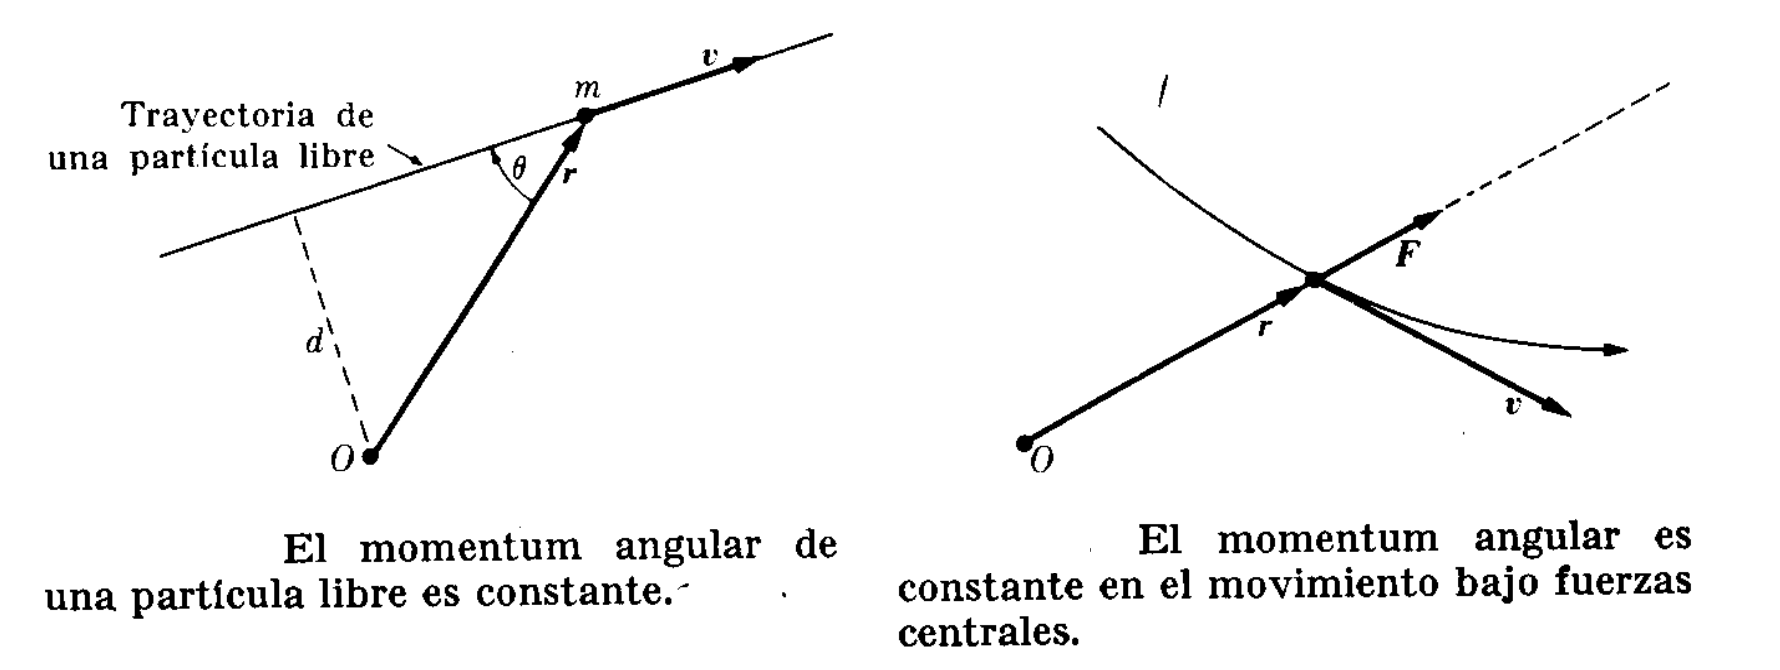
\includegraphics[width=1\textwidth]{imagenes/imagenes04/T04IM20.png}
\end{figure}


\begin{miparrafo}
	
	\textbf{---} $\overrightarrow{M}=\vec 0 \text { si } \vec F=\vec 0$. \emph{Partícula libre}, $L=mvr\sin \theta =mvd=cte \to v=cte \ : \ $ \emph{movimiento rectilíneo}.
	
	\textbf{---} $\overrightarrow{M}=\vec 0 \text { si } \vec F \;||\; \vec r,\ \text{ si } \vec F \text{ pasa por } \mathcal O \to \vec F \ $ \emph{es fuerza central}.

	\emph{Si un cuerpo se mueve bajo la acción de una fuerza central, su momento angular es un vector constante, $\overrightarrow{L}=\overrightarrow{cte}$ (y viceversa).} \textsf{Resultado importante, muchas fuerzas de la naturaleza son centrales.}

\end{miparrafo}	


\begin{ejem} Como hemos visto antes, $L=\displaystyle m r^2 \dv{\theta}{t}$. En fuerzas centrales (gravitación) $\displaystyle L=cte \to r^2 \dv{\theta}{t}=cte$

\begin{multicols}{2}
En radianes, \emph{arco=ángulo x radio}, $\dd s = r \dd \theta$.

El área de un sector circular de ángulo $\dd \theta$ es $\ \dd A= \frac 1 2 r^2 \dd \theta$. 

$\displaystyle \dv{A}{t}=\frac 1 2 r^2 \dv{\theta}{t}=cte$, luego,

 \textbf{``en movimientos bajo fuerzas centrales, el radio-vector de la partícula barre áreas iguales en tiempos iguales.\footnote{Histórica ley de Keppler.}}
\begin{figure}[H]
	\centering
	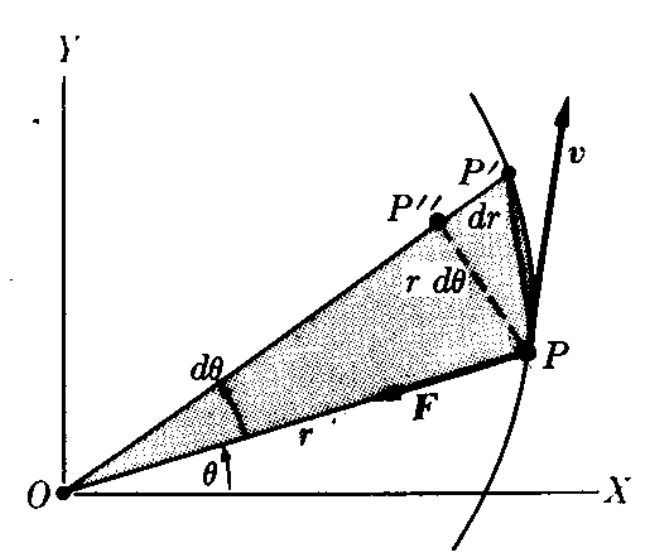
\includegraphics[width=0.5\textwidth]{imagenes/imagenes04/T04IM21.png}
\end{figure}
\end{multicols}
\end{ejem}



\begin{ejem}{Movimiento unidimensional en un campo conservativo}
	
$\mathcal E=\mathcal E_c+\mathcal E_p=\dfrac 1 2 m v^2 + \mathcal E_p=cte$

$\dfrac 1 2 m \displaystyle \left( \dv{x}{t} \right)^2 = \mathcal E-\mathcal E_p \to \dv{x}{t}=\sqrt{\dfrac 2 m} \ \sqrt{\mathcal E-\mathcal E_p}$

$\displaystyle \dfrac {\dd x}{\sqrt{\mathcal E-\mathcal E_p}}=\sqrt{\dfrac 2 m} \ \dd t$

 $\displaystyle \vec F=-\overrightarrow{ \grad{\mathcal E_p}}\to F=-\dv{\mathcal E_p}{x}=0 \Rightarrow \mathcal E_p=cte $. Movimiento uniforme.
 
 Integrando y teniendo en cuenta que $\mathcal E-\mathcal E_p=\mathcal E_c$
 
 $\displaystyle \boldsymbol{ x}=x_0+ \sqrt{\dfrac 2 m}\ \mathcal E_c^{1/2} \ t=
 x_0 + \sqrt{\dfrac {\cancel{2}}{\bcancel{m}}} \ \sqrt{\dfrac 1 {\cancel{2}} \ \bcancel{m} \ v_0^2} \ t \boldsymbol{ = x_0+v_0\ t}$
 
 \textbf{Ejercicio:} Determinar la ley de movimiento unidimensional en que $F=cte$, Ha de salir la ley del MRUA.	
 \end{ejem}
\footnotesize{\textcolor{gris}{$F=cte \to a=F/m=cte \to \dv{v}{t}=a=cte \to v=v(t)=\dv{x}{t}\to  x=x(t)$; MRUA}}\normalsize{.}



\section{Campos de fuerza no conservativos}


En campos conservativos: $\Delta \mathcal E=\Delta (\mathcal E_c + \mathcal E_p)= 0$

Pero también existen campos de fuerza no conservativo, en este caso:

$\vec F_{total}=\vec F_{conservativa}+\vec F_{no\ conservativa}=\vec F_c+ \vec F_{NC}$

En estas condiciones, el trabajo elemental para trasladar a un cuerpo desde un punto a uno infinitamente próximo será:

$\vec F_{total} \cdot \dd \vec r=\dd \mathcal E_c$

$\dd \mathcal E_c=(\vec F_C+\vec F_{NC})\cdot \dd \vec r=\vec F_C\cdot \dd \vec r+\vec F_{NC} \cdot \dd \vec r=-\dd \mathcal E_p + \vec F_{NC}\cdot \dd \vec r$

$\dd \mathcal E_c+\dd \mathcal E_p=\boldsymbol{ \dd (\mathcal E_c+\mathcal E_p)=\dd \mathcal E=\vec F_{NC}\cdot \dd \vec r }$

Integrando:

\begin{equation}
\subrayado{\Delta (\mathcal E_c+\mathcal E_p)=W_{NC}	}
\end{equation}

En el caso de comparar dos estados:

\begin{equation}
{(\mathcal E_c+\mathcal E_p)}_2-{(\mathcal E_c+\mathcal E_P)}_1=W_{NC}	
\end{equation}

Vamos a restringir el problema al caso de que el $W_{NC}$ sea debido a las fuerzas de fricción (rozamiento).

\begin{multicols}{2}
La fuerza de rozamiento $\vec F_R$ y el desplazamiento $\dd \vec r$ forman un ángulo de $180^o$ (\textit{la fuerza de rozamiento siempre es opuesta al movimiento}).
\begin{figure}[H]
	\centering
	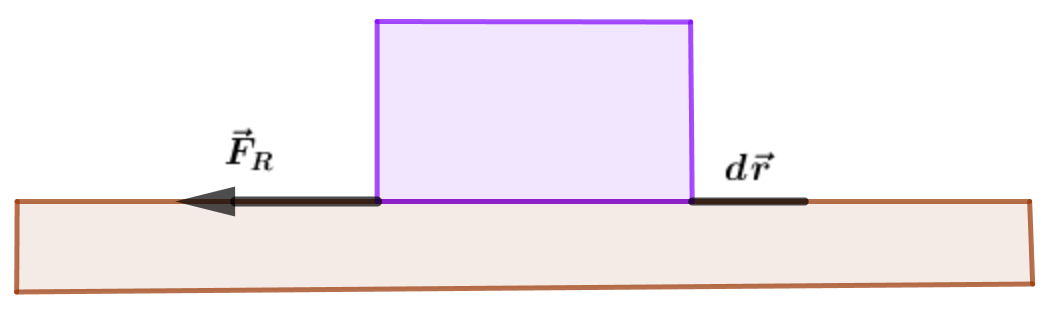
\includegraphics[width=0.4\textwidth]{imagenes/imagenes04/T04IM04.png}
\end{figure}
\end{multicols}
$W_{NC}=\displaystyle \int_1^2 \vec F_R\cdot \dd \vec r=-\int_1^2 F_R\ \dd r=-F_R\ (r_2-r_1) \Rightarrow W_{NC}<0$

$\Delta (\mathcal E_c+\mathcal E_p)=W_{NC} \to {(\mathcal E_c+ \mathcal E_p)}_2<{(\mathcal E_c+\mathcal E_p)}_1 \Rightarrow \mathcal E_2 < \mathcal E_1$

\textbf{?`Dónde está la energía que falta? $\longrightarrow $ CALOR }

Para este caso particular de trabajo no conservativo debido a fuerzas de fricción:  $W_{NC}=-\mathcal Q \rightarrow \boldsymbol{ \Delta \mathcal E+\mathcal Q=0 }$

\emph{En campos no conservativos debido a fuerzas de fricción, la energía mecánica no se conserva, parte de ella se disipa en forma de calor.}

\vspace{-4mm}\section{Conservación de la energía}

\vspace{-4mm}$$\mathcal E=\mathcal E_c+\mathcal E_p;\qquad \Delta \mathcal E=W_{NC}$$
$$\subrayado{\Delta \mathcal E_c + \Sigma \Delta \mathcal E_p=W_{NC}}$$,

donde con $\Sigma \Delta \mathcal E_p$ queremos indicar la contribución al trabajo de \emph{todas} las fuerzas conservativas presentes (gravitatoria, eléctrica, elástica, electromagnética, nuclear, ...)

\begin{equation}
	\Delta \mathcal E_c + \Sigma \Delta \mathcal E_p + \mathcal Q+\text{ \small{(el  cambio  en  otras  formas  de  energía)} }= 0
\end{equation}

\vspace{-4mm}Principio de conservación de la energía: \emph{La energía total de un sistema físico se conserva. La $\mathcal E_{total}$ es constante. La energía puede transformarse de una clase a otras, pero no puede ser creada ni destruida.}

\begin{figure}[H]
	\centering
	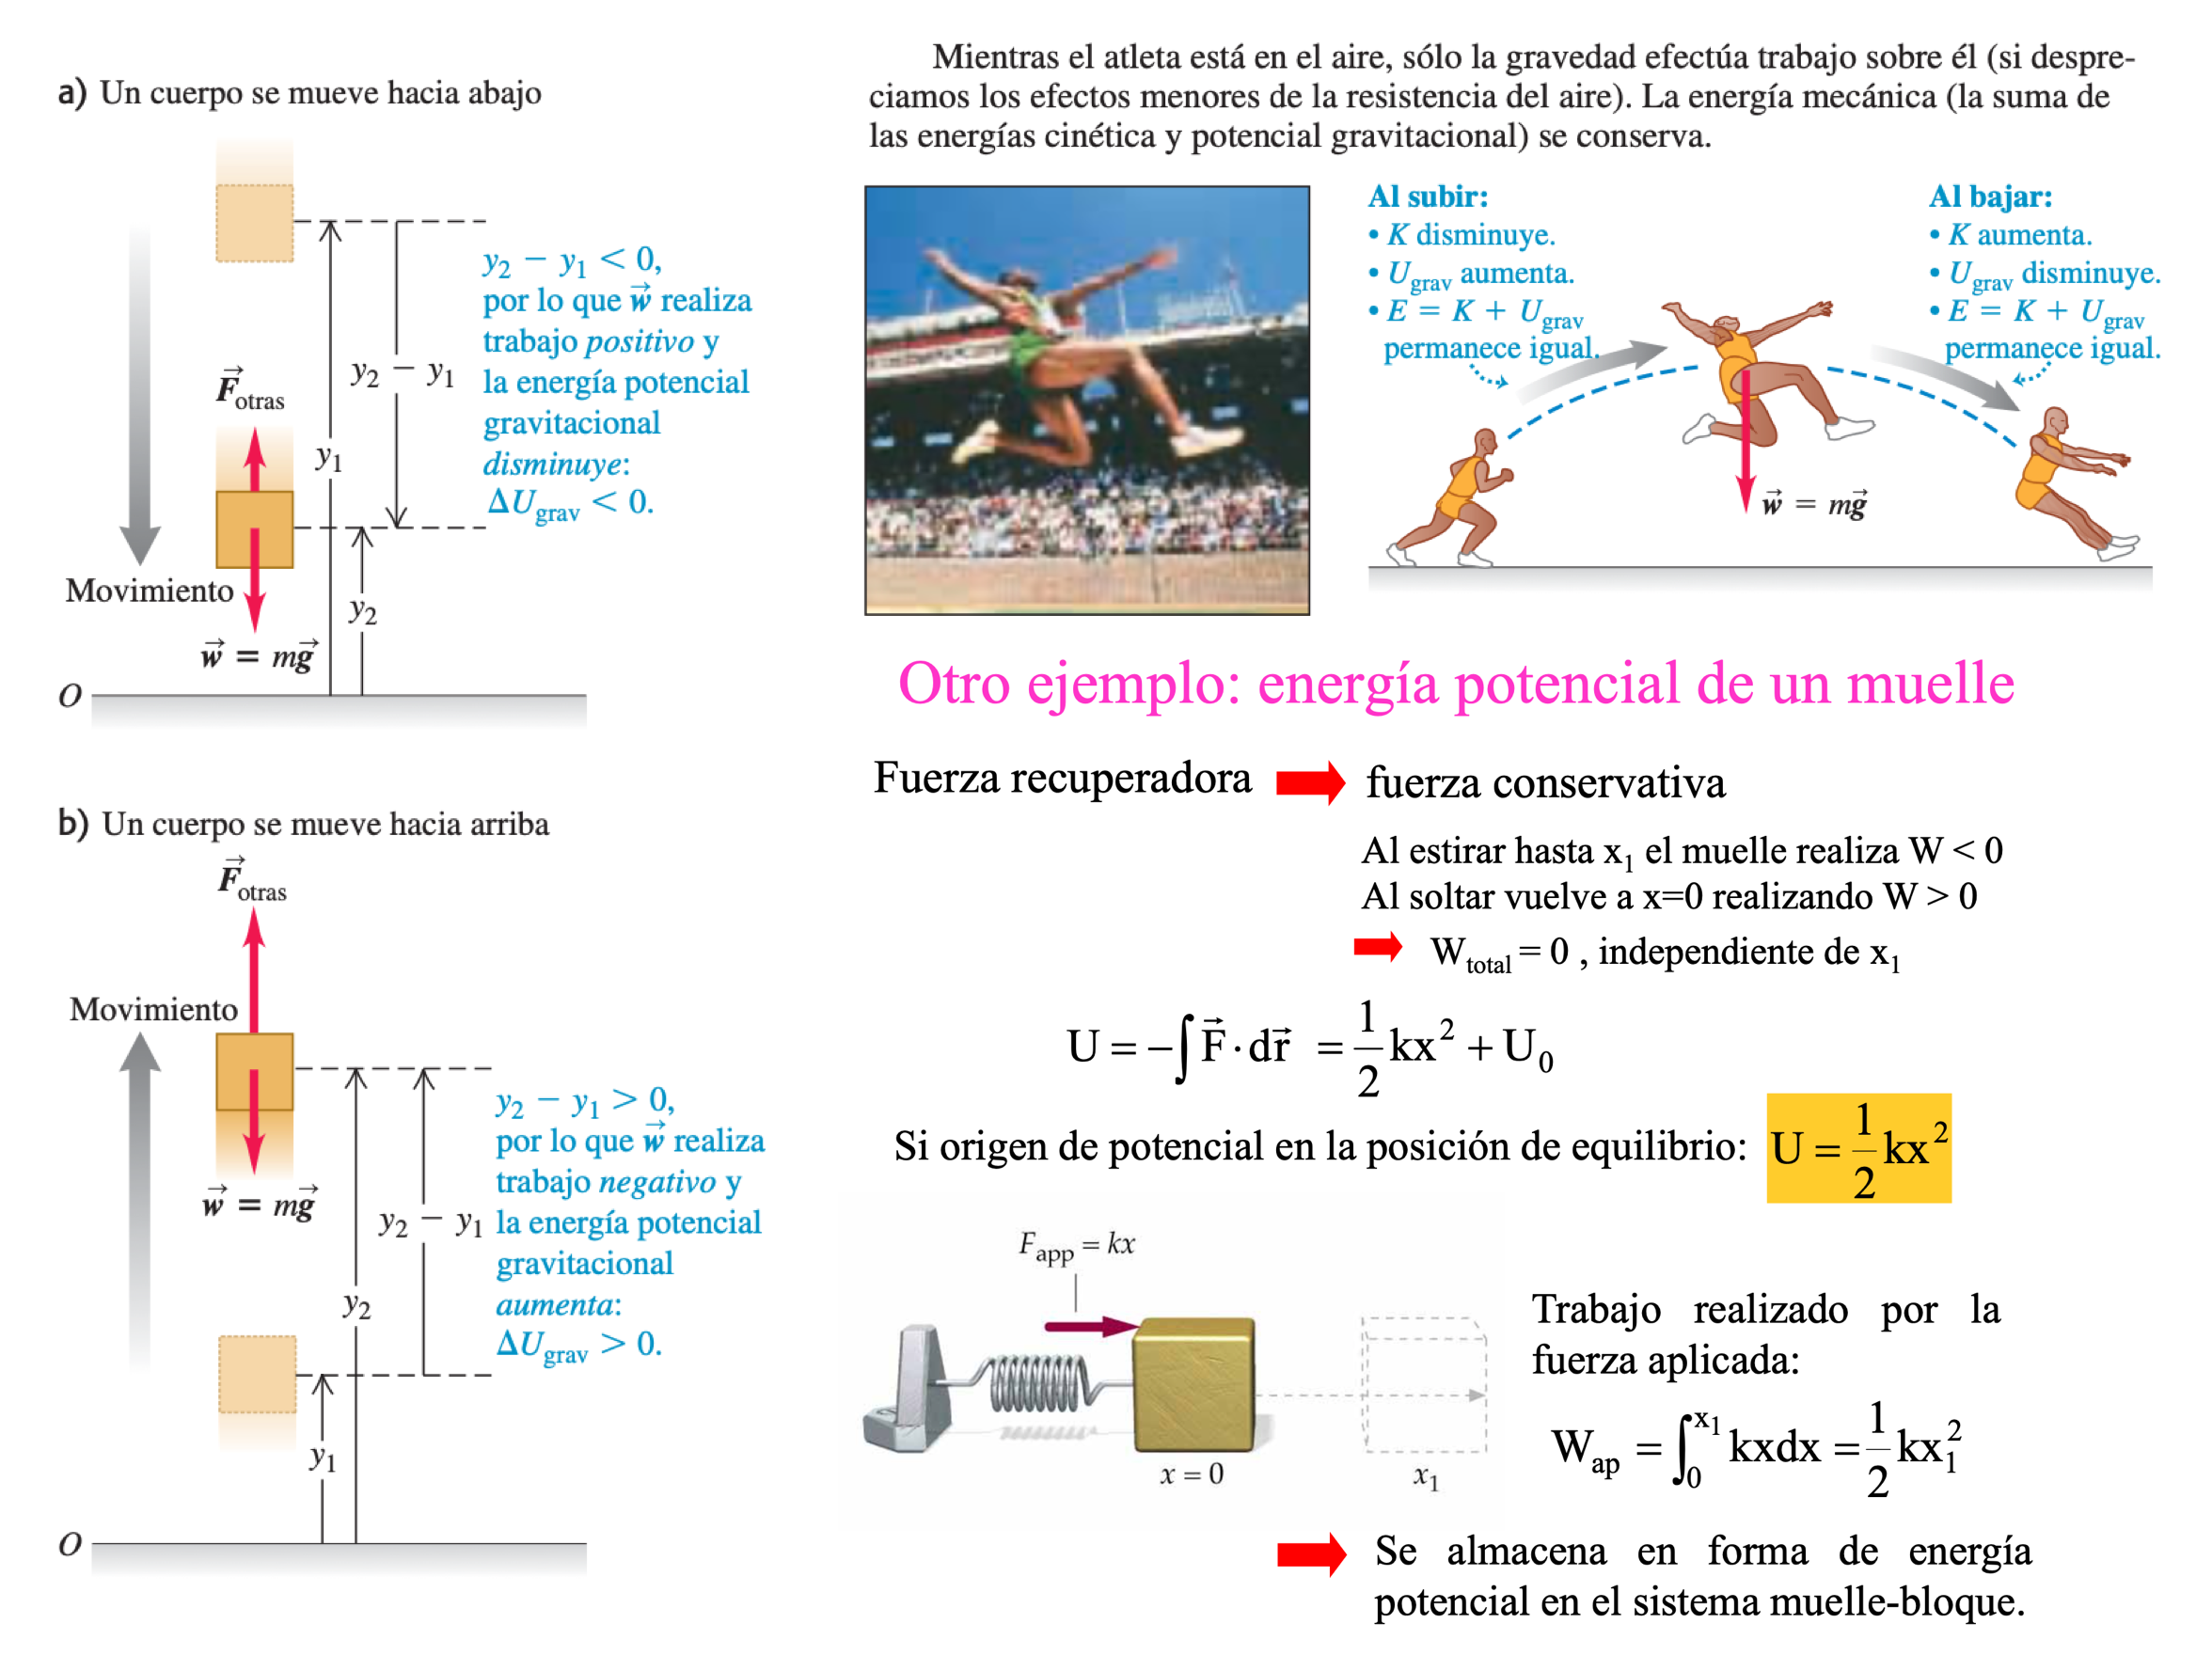
\includegraphics[width=1\textwidth]{imagenes/imagenes04/T04IM05.png}
\end{figure}

\begin{figure}[H]
	\centering
	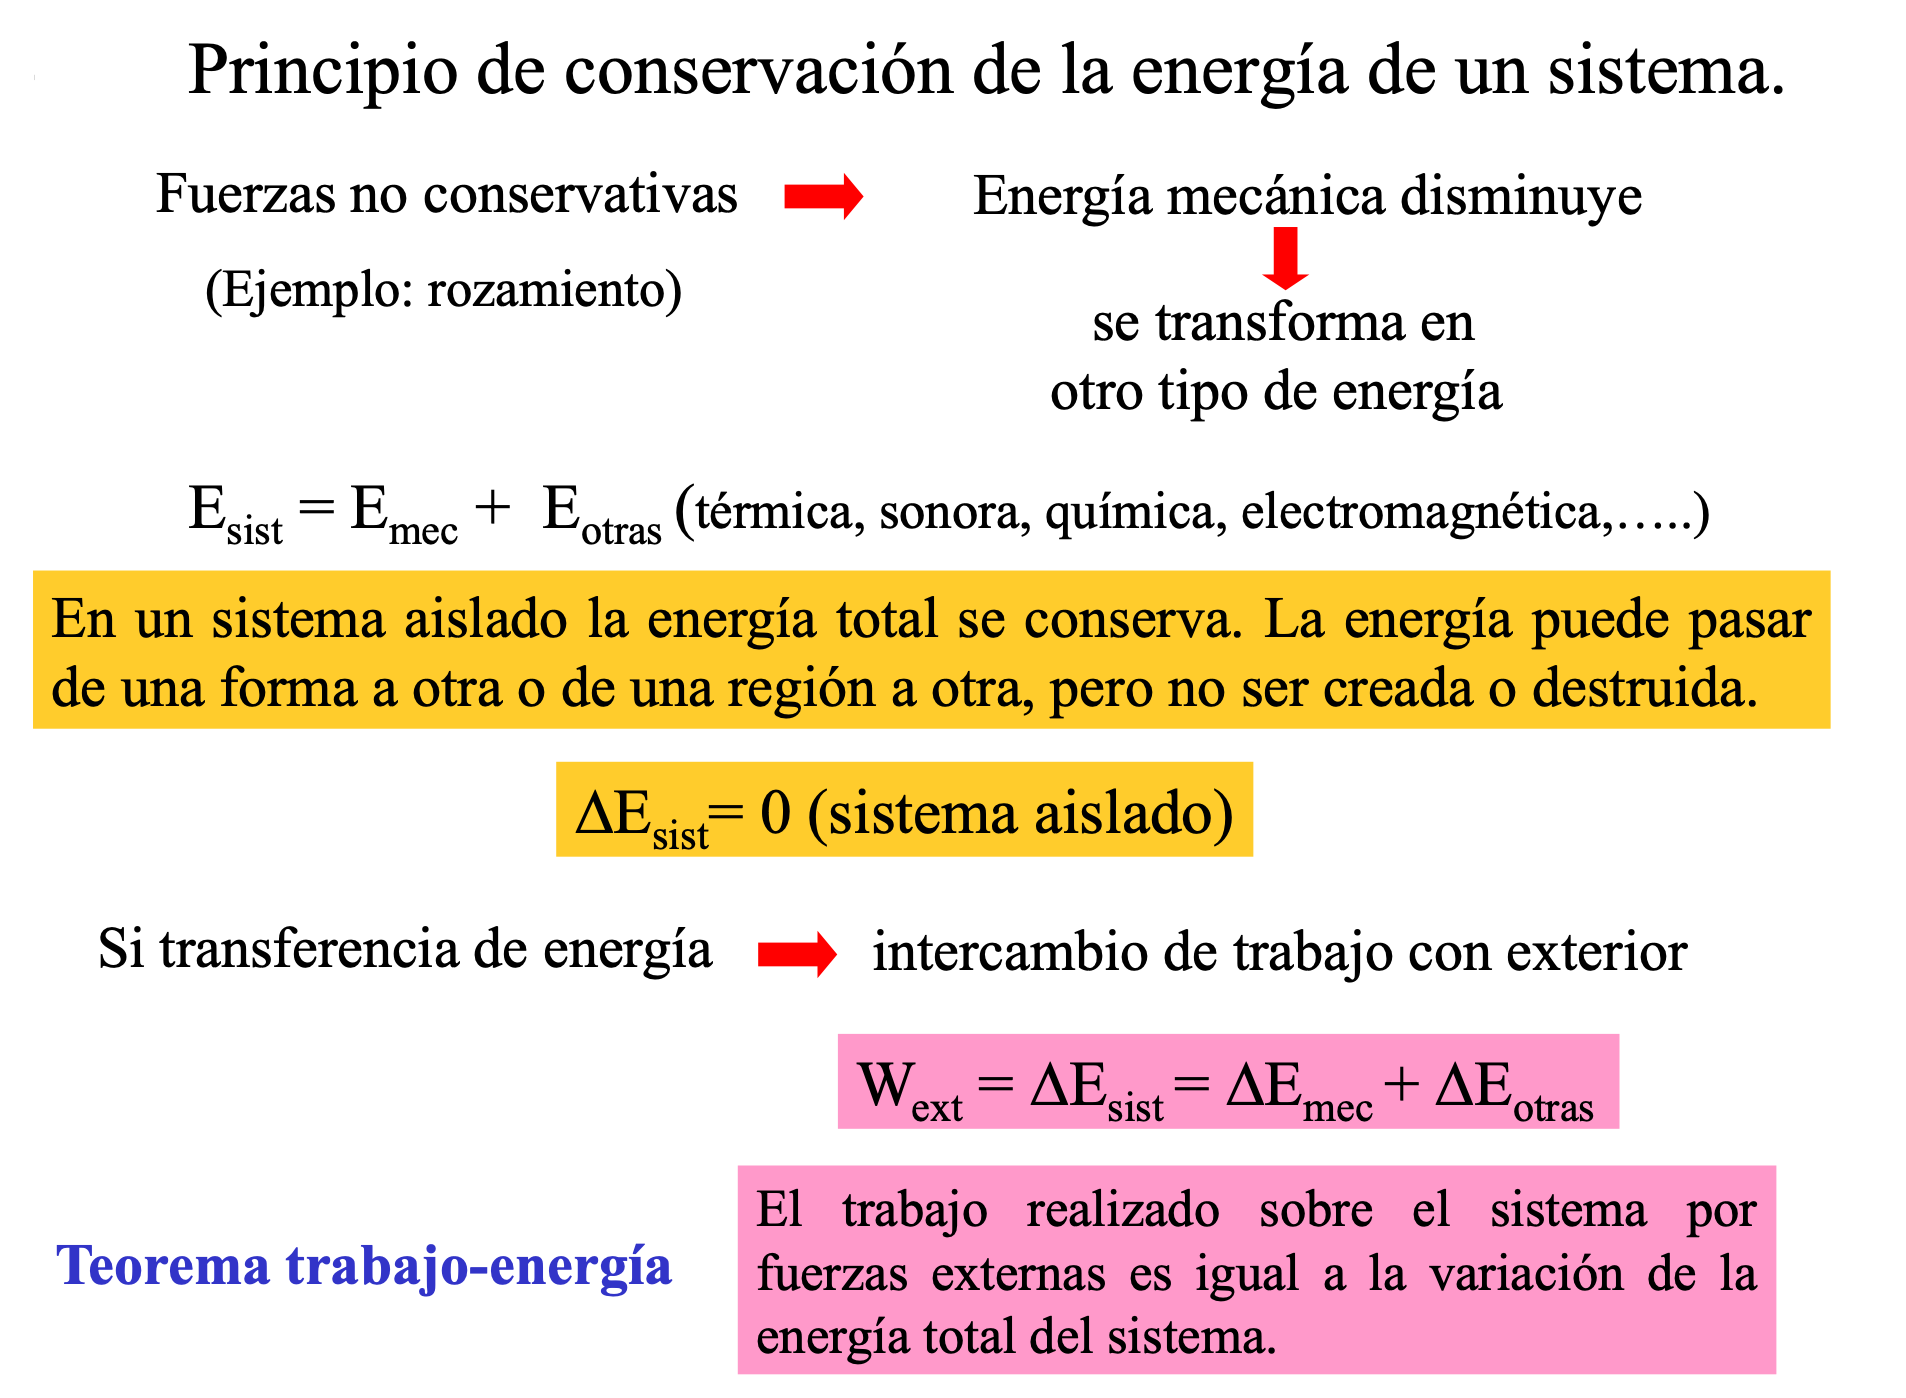
\includegraphics[width=1\textwidth]{imagenes/imagenes04/T04IM11.png}
\end{figure}


\newpage %***************************
\section{Problemas}

\begin{prob}
Una partícula se mueve bajo la acción de una fuerza atractiva que varía inversamente al cuadrado de la distancia, $F=-K/r^2$. La trayectoria de la partícula en una circunferencia de radio $r$. Calcúlese, en función de $k$ y $r$, la energía total, la velocidad y el momento angular de la partícula en cada instante.	
\end{prob}

$\vec F=-\dfrac k {r^2}\ \vec u_r ; \qquad \vec F \cdot \dd \vec r=-\dd \mathcal E_p \to --\dfrac k {r^2} \vec u_r \cdot \dd \vec r=-\dd \mathcal E_p \to$

Tomamos el origen de energía potencial en el infinito:

$\displaystyle \int_{\infty}^r \dfrac k {r^2} \dd r = \int_0^{\mathcal E_p} \dd \mathcal E_p \to -\dfrac k r =\mathcal E_p \Rightarrow \quad \mathcal E_p(r)=-\dfrac k r$


$\mathcal E_c=\dfrac 1 2 m v^2=\dfrac 1 2  \left( m \dfrac {v^2} r \right)  r \to \ $ el movimiento es en una circunferencia, luego $F=m\dfrac {v^2}r$, además, como \textbf{la $\boldsymbol{\mathcal E_c}$ es siempre positiva}, tenemos que:

$\displaystyle \mathcal E_c=\dfrac 1 2 \ (F) \ r=\dfrac 1 2 \dfrac k {r^2} r=\dfrac 1 2 \dfrac k r$

Por lo que $\ \mathcal E=\mathcal E_c+\mathcal E_p=\dfrac 1 2 \dfrac k r - \dfrac k r = - \dfrac 1 2 \dfrac k r$, constante en cada órbita.

Calculemos la velocidad de la partícula: $\dfrac 1 2 m v^2 = \textcolor{gris}{\mathcal E_c}=\dfrac 1 2 \dfrac k r \to $

$\displaystyle mv^2=\dfrac k r \Rightarrow v=\sqrt{\dfrac k {rm}}$, constante en cada órbita.

Momento angular: $\vec L=\vec r \times \vec p=\vec r \times m \vec v \to L=mrv \sin 90^0=mrv \Rightarrow$

$L=mr\sqrt{\dfrac k{rm}}=\sqrt{krm}$, constante en cada órbita.

\begin{prob}
Una partícula de masa $m$ se encuentra en un campo central de valor $\vec F=-3x^3\vec i \ \mathrm{N}$, si $x$ se expresa en $\mathrm{m}$. Sabiendo que la energía total es de $8\ \mathrm{J}$, determinar la región del espacio unidimensional en la que puede moverse la partícula de acuerdo con la ley de conservación de la energía.	
\end{prob}
$\displaystyle \vec F=-3x^3\vec i =-\overrightarrow{\nabla} \mathcal E_p=-i\ \dv{\mathcal E_p}{x} \to$ tomando el origen de energía potencial en el centro del campo, $x=0 \to \displaystyle \mathcal E_p=\int_0^{\mathcal E_p} \dd \mathcal E_p=\int_0^x 3x^3 \dd x=\dfrac 3 4 x^4$

$\mathcal E=\mathcal E_c+\mathcal E_p \to \mathcal E\mathcal {E_p}_{max} \to 8=\dfrac 3 4 x_{max}^4 \to x_{max}=\pm 1.807\ \mathrm{m}$

La partícula se puede mover de modo que  $-1.807 < x (\mathrm{m}) < 1.807$, la región de movimiento de la partícula es el intervalo $[-1,807,1.807]\ \mathrm{m}$. 



\begin{prob}
Un skater baja en monopatín por una rampa curva en un parque. Tratado puntualmente como una partícula, describe un círculo de radio $R=3\ \mathrm{m}$. La masa total de joven skater y su monopatín es de $25\ \mathrm{kg}$. El movimiento parte del reposo y no hay fricción. Calcúlese la velocidad en la base de la rampa así como la fuerza normal que actúa sobre él en ese momento.	
\end{prob}
\vspace{-4mm}\begin{figure}[H]
	\centering
	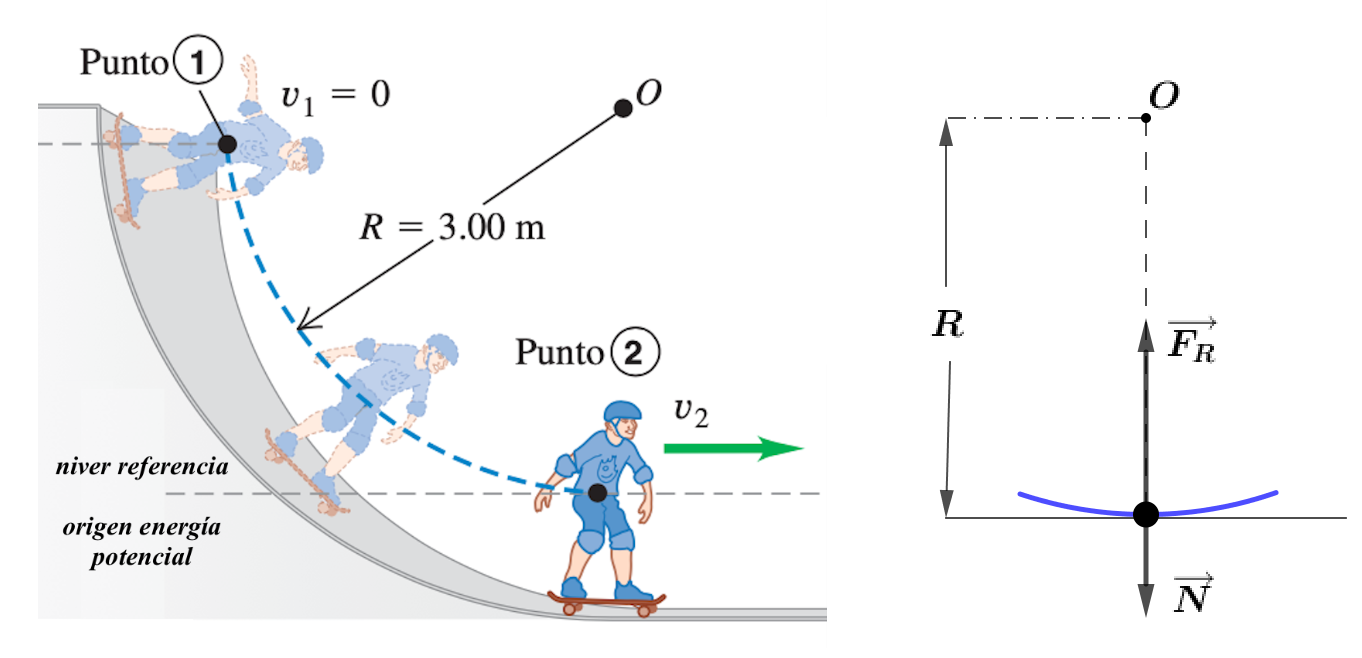
\includegraphics[width=1\textwidth]{imagenes/imagenes04/T04IM14.png}
\end{figure}
 $  \nexists F_R \to \mathcal E \ $ se conserva, $\ \mathcal E_1=\mathcal E_2$
 
 $\mathcal E_{c_1}+\mathcal E_{p_1}=\mathcal E_{c_2}\mathcal E_{p_2} \to 0+mgR=\frac 1 2 m v^2 +0 \to v=\sqrt{2gR}=7.67\ \mathrm{ms}^{-1}$
 
 $\Sigma F_y=ma_y$; $\quad a_y=a_n=\dfrac {v^2}{R}=\dfrac{2gR}{R}=2g; \quad \Sigma F_y=N-mg$, donde hemos asignado sentido positivo el que va hacia arriba en el eje $Y$.
 
 $N-mg=2mg \to \quad N=3mg=735\ \mathrm{N}$
 
 \begin{prob}
 	Si el niño skater tan solo alcanza los $6.00 \ \mathrm{ms}^{-1}$ en la base de la rampa debido a fuerzas de fricción, ?`cuál es el trabajo desarrollado por éstas?
 \end{prob}
 

 \vspace{-3mm}$\Delta \mathcal E_p=0-mgh=-735\ \mathrm{J}; \qquad \Delta \mathcal E_c=\frac 1 2 m v^2-0=450\ \mathrm{J}$
 
  $ W_{NC}=\Delta \mathcal E = \Delta \mathcal E_p+\Delta \mathcal E_p\textcolor{gris}{=-735+450}=-285\ \mathrm{J}$
  
  El rozamiento ha causado una disminución de $285\ \mathrm{J}$ en la energía mecánica.
 
 
 
 \begin{prob}.
	\begin{figure}[H]
	\centering
	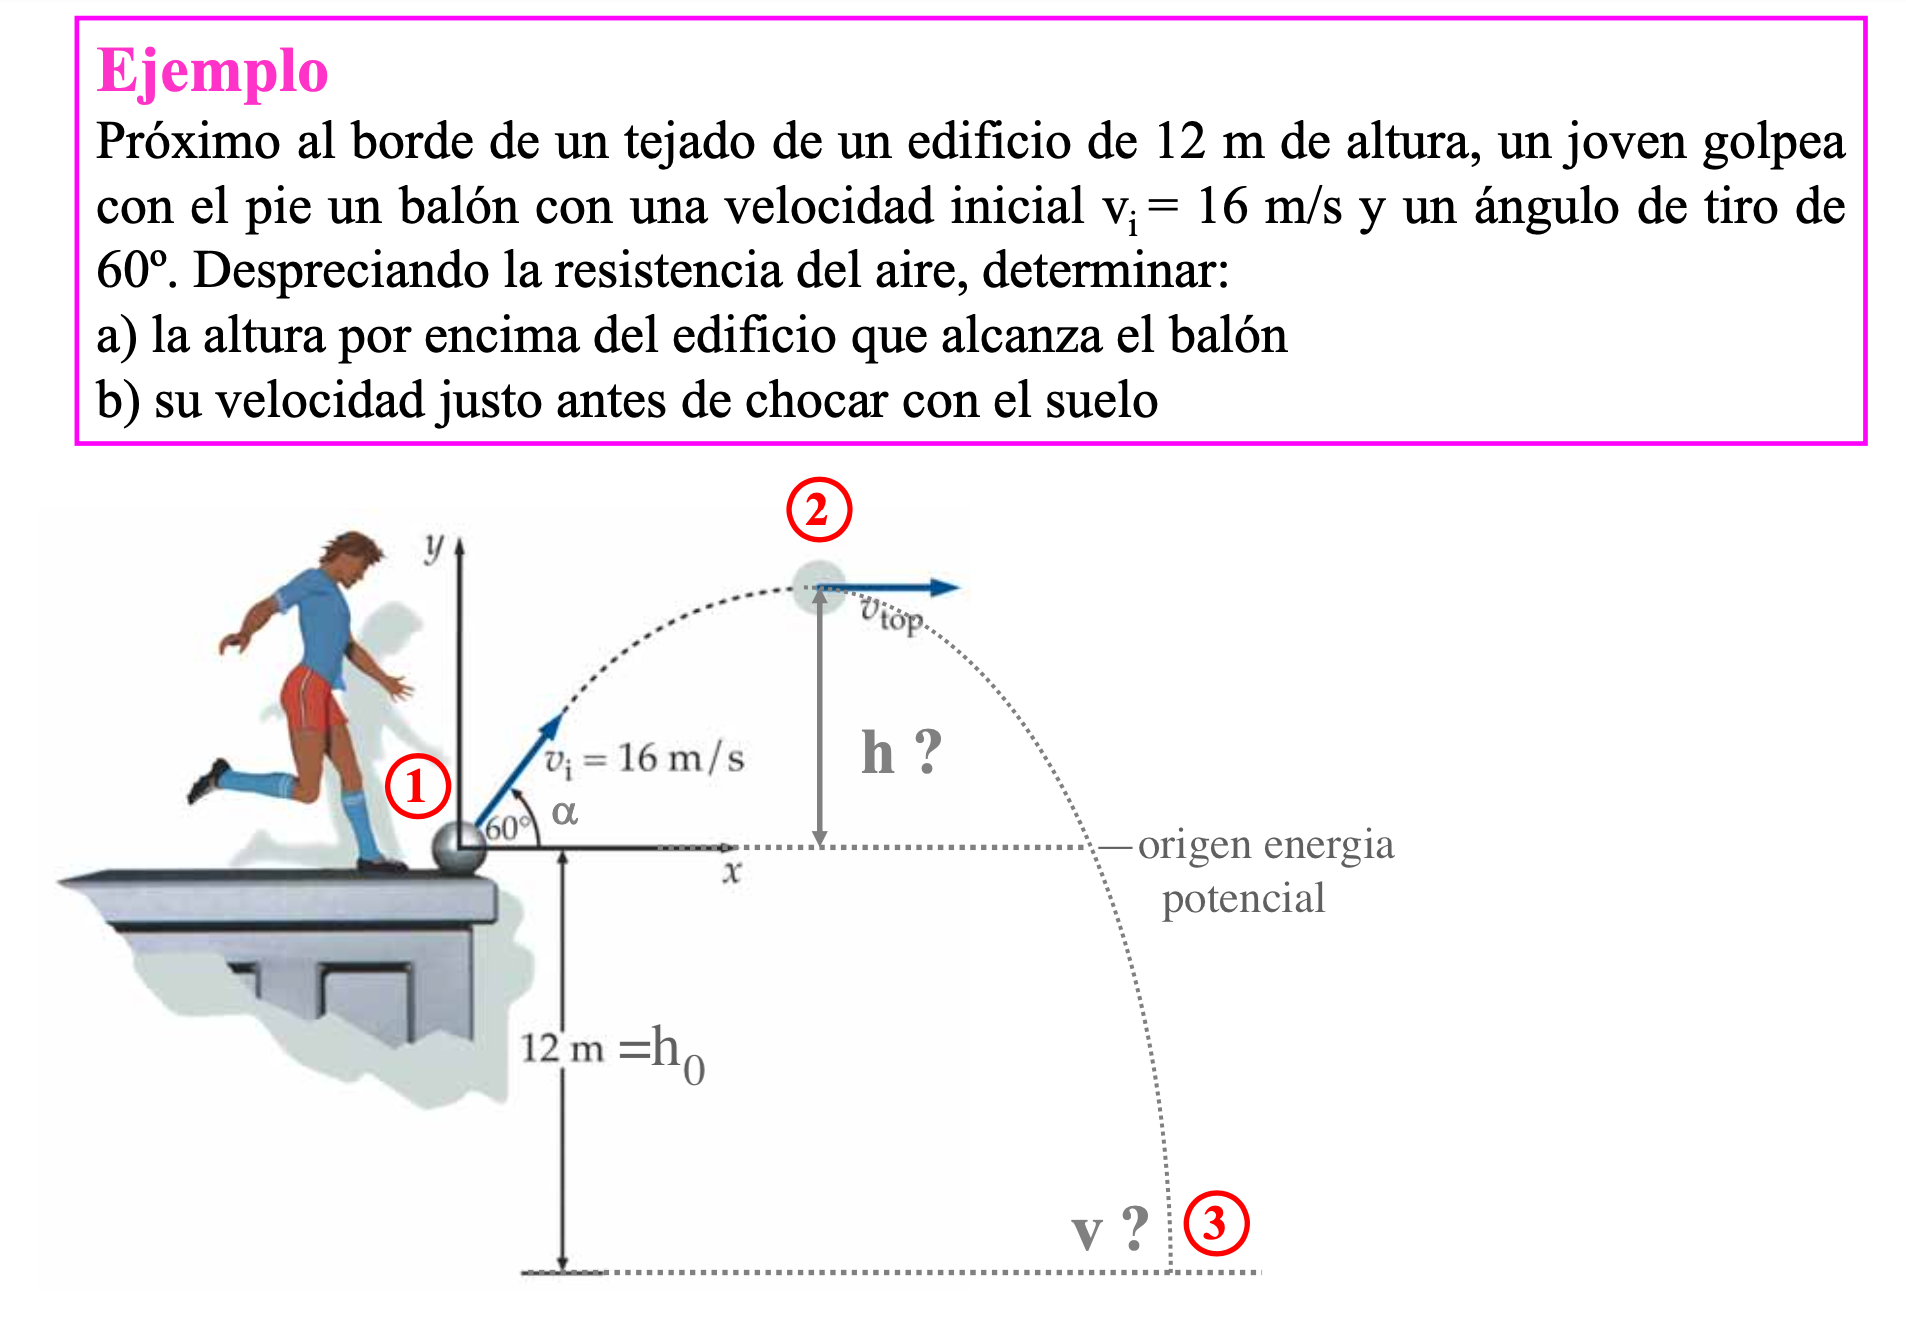
\includegraphics[width=1\textwidth]{imagenes/imagenes04/T04IM06.png}
\end{figure}
\end{prob}

 $  \nexists F_R \to \mathcal E \ $ se conserva, $\ \mathcal E_1=\mathcal E_2$
 
 $1)\quad \mathcal E_c=\frac 1 2 m v_i^2; \quad  \mathcal E_p=mgh_0 $
 
 $2)\quad \mathcal E_c=0; \quad  \mathcal E_p=mg(h_0+h)$
 
 $ \mathcal E_1= \mathcal E_2 \to h=\dfrac {v_0^2}{2g}$
 
 $3) \mathcal E_c=\frac 1 2 m v^2; \quad  \mathcal E_p=0$
 
 $  \mathcal E_1= \mathcal E_3 \to v=\sqrt{v_o^2+2gh_o}$
 
 \textbf{análisis de casos límites:} si $h_0=0 \to v=v_0$ y $h$ son la velocidad de llegada y la altura máxima de tiro parabólico en superficie horizontal desde el suelo.



\begin{prob}
Un cuerpo de masa $m$ cuelga de un hilo de longitud $L$ y masa despreciable. La partícula se deslaza un ángulo $\theta_0$ de la vertical y se suelta. Encontrar la velocidad en el punto más bajo, en un punto intermedio, en su simétrico, la tensión del cable cuando la partícula está en el punto más bajo y el ángulo para el cual la velocidad es la mitad de la velocidad máxima.
\end{prob}

Las únicas fuerzas que actúan son el peso y la tensión en la cuerda. La variación de energía cinética es el trabajo realizado, la tensión siempre es perpendicular al desplazamiento por lo que no efectúa trabajo. La fuerza peso es conservativa por lo que el trabajo que desarrolla es igual a menos la variación de la energía potencial. Luego $\Delta \mathcal E_c=W=-\Delta \mathcal E_p \to \Delta \mathcal E=0$, la energía se conserva, $\mathcal E_i=\mathcal E_f$.


Al soltar la partícula la masa bajo la acción del peso y la tensión de la cuerda, describirá un arco de círculo de radio $L$ pasando por la vertical (su punto más bajo, $2$) y sigue moviéndose hacia la izquierda hasta llegar a una posición simétrica a la inicial (ángulo $-\theta$). A partir de ahí el movimiento se repite de un lado a otro resultando las \emph{oscilaciones de un \textbf{péndulo}}.


%\newpage %*************************************************
\begin{multicols}{2}

Balance energético en los puntos $1$, un punto intermedio y $2$:

$\begin{cases}
\mathcal E_{c_1}=0 & \mathcal E_{p_1}=mgL(1-\cos \theta_0) \\
\mathcal E_{c}=\frac 1 2 m v^2 & \mathcal E_{p}=mgL(1-\cos \theta) \\
\mathcal E_{c_2}=\frac 1 2 m v_{max}^2 & \mathcal E_{p_1}=0
\end{cases}$

$\mathcal E = \mathcal E_c+\mathcal E_p$
	\begin{figure}[H]
	\centering
	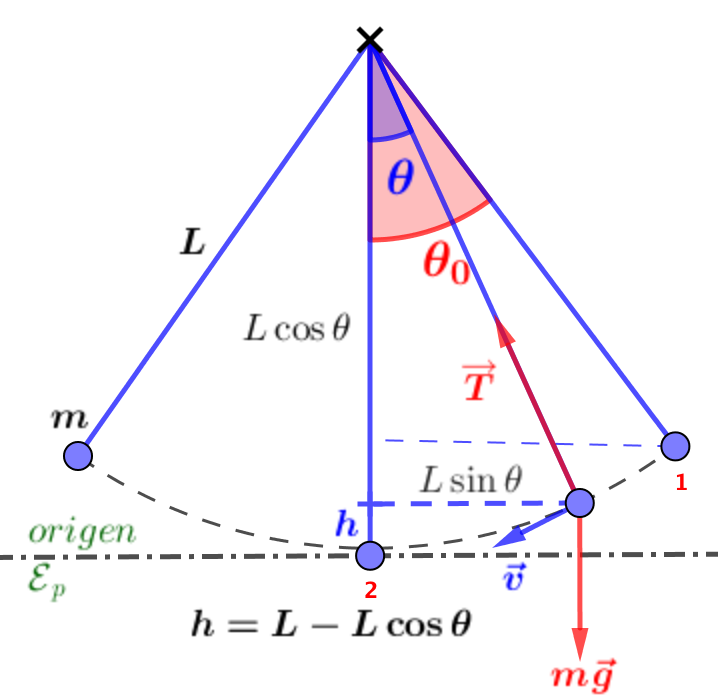
\includegraphics[width=.4\textwidth]{imagenes/imagenes04/T04IM15.png}
\end{figure}
\end{multicols}
--- Velocidad en el punto más bajo, $2$: $\mathcal E_1=\mathcal E_2 \to mgL(1-\cos \theta_0)=\frac 1 2 m v_{max}^2 \quad \to \qquad v_{max}=\sqrt{2gl(1-\cos \theta_0)}$

--- Velocidad en un punto intermedio: $\mathcal E=\mathcal E_1 \to \frac 1 2 m v^2+mgL(1-\cos \theta= mgL(1-\cos \theta_0) \quad \to \qquad v=\sqrt{2gl(\cos \theta-\cos \theta_0)}$

--- Velocidad en el punto simétrico: el ángulo será $\theta$, como $\cos (-\theta)=\cos \theta \to $ la velocidad es la misma que la calculada en el punto anterior.

--- Tensión en el punto más bajo de la trayectoria: $T-mg=ma=ma_N=m\dfrac {v^2}{L}=m\dfrac{v_{max}^2}{L}=m\dfrac{2gL(1-\cos \theta_0)}{L} \quad \to \qquad T=mg\left[ 3-2-\cos \theta_0 \right]$

--- Ángulo con la vertical cuando $v=\frac {1}{2}v_{max} \to  \sqrt{2gl(\cos \theta-\cos \theta_0)}=\sqrt{2gl(1-\cos \theta_0)}$, despejando: 

$ cos \theta=\dfrac {1-4\cos \theta_0}{5} \to  \theta= \arccos \left( \dfrac {1-4\cos \theta_0}{5}\right)$


\begin{prob}
\begin{multicols}{2}
Determinar la altura mínima desde la cual una bola se debería soltar para que pueda \emph{``rizar el rizo''}, completar el movimiento mostrado en la figura adjunta. Se supone que la bola se desliza sin rodar y que no hay rozamiento.	
\begin{figure}[H]
	\centering
	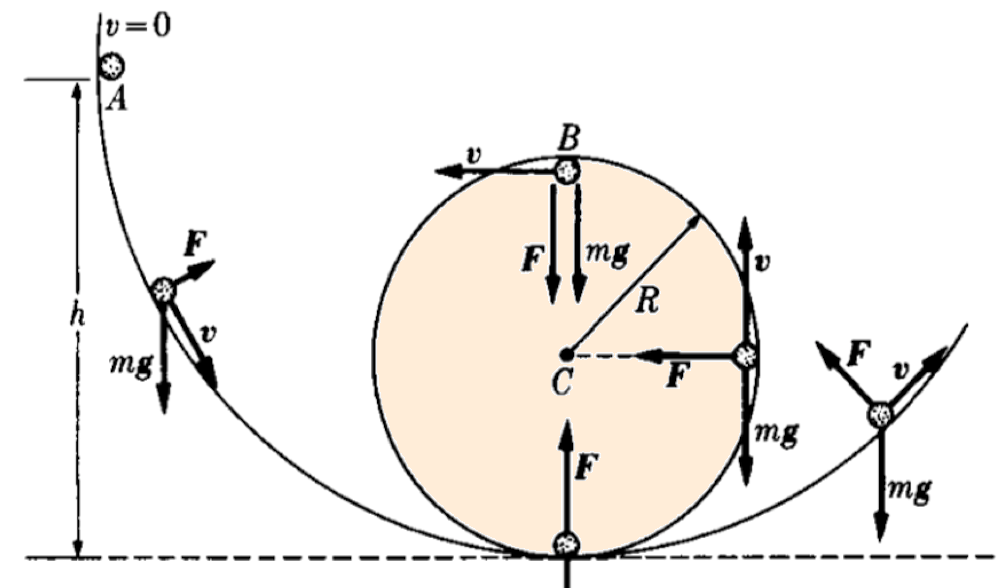
\includegraphics[width=.55\textwidth]{imagenes/imagenes04/T04IM16.png}
\end{figure}
\end{multicols}
\end{prob}
Supongamos que la bola se suelta en $A$, a una altura $h$ sobre la base de la circunferencia (\emph{rizo}). La bola baja ganando velocidad y empieza a perderla cuando sube por el rizo. Las fuerzas que actúan son el peso y la reacción normal del riel $F$, que siempre apunta hacia el centro del rizo cuando la bola se encuentra dentro de este. 

Se conserva la energía pues no hay rozamiento y la única fuerza que produce trabajo es el peso $mg$.

En el punto más alto del rizo, $B$, tenemos:

$\Sigma F_y=mg+F=ma_y=ma_N=m\dfrac {v^2}R$

La velocidad mínima en $B$ para `rizar el rizo' ocurrirá cuando $F=0   \to mg=m\dfrac {v^2}R \to \ v=\sqrt{gR}$

Si $v < \sqrt{gR} \to mg>F_N $ y la bola se separa del riel y cae describiendo una parábola.

Para calcular la altura $h$ correspondiente establecemos un balance energético en tos puntos $A$ y $B$, es decir, usamos que al conservarse la energía, $\mathcal E_A=\mathcal E_B$

$\mathcal E_A=\mathcal E_{c_A}+\mathcal E_{p_A}=0+mgh=mgh$

En $B,\quad y=2R; \; v^2=gR$, luego:

$\mathcal E_B=\mathcal E_{c_B}+\mathcal E_{p_B}=\frac 1 2 m (gR) + mg(2R)=\frac 5 2 mgR$

Igualando: $h= 5 / 2 R$, es la mínima altura para `rizar el rizo'. Esto es así si no hay fuerzas de rozamiento y si la bola se desliza sin rodar (como una partícula). Si la bola rueda hay que considerarla como un sólido rígido y se estudiará en un tema más adelante.



\begin{prob}
	Un bloque de $4 \ \mathrm{kg}$ cuelga de una cuerda ligera a través de una polea sin rozamiento y de masa despreciable que está conectada a un bloque de $ 6 \ \mathrm{kg}$ que descansa sobre una plataforma horizontal. El coeficiente de rozamiento es $\mu=0.2$. El bloque de $6 \ \mathrm{kg}$ se empuja contra un muelle de constante $k=180\ \mathrm{Nm}^{-1}$ que se comprime $30 \ \mathrm{cm}$. Determinar la velocidad de los bloques cuando el muelle se libera y el bloque de $4 \ \mathrm{kg}$ cae una distancia de $40 \ \mathrm{cm}$.
\end{prob}

Al haber fuerzas de fricción, se cumplirá que $\Delta \mathcal E=W_{NC}$.
\begin{multicols}{2}

Intervienen tres tipos de energia cinética, potencial gravitatoria y potencial elástica.

Compararemos las energías mecánicas en dos puntos: 1, cuando comprimimos el muelle y 2, cuando el cuerpo de $4 \ \mathrm{kg}$ pende $40\ \mathrm{cm}$.
\begin{figure}[H]
	\centering
	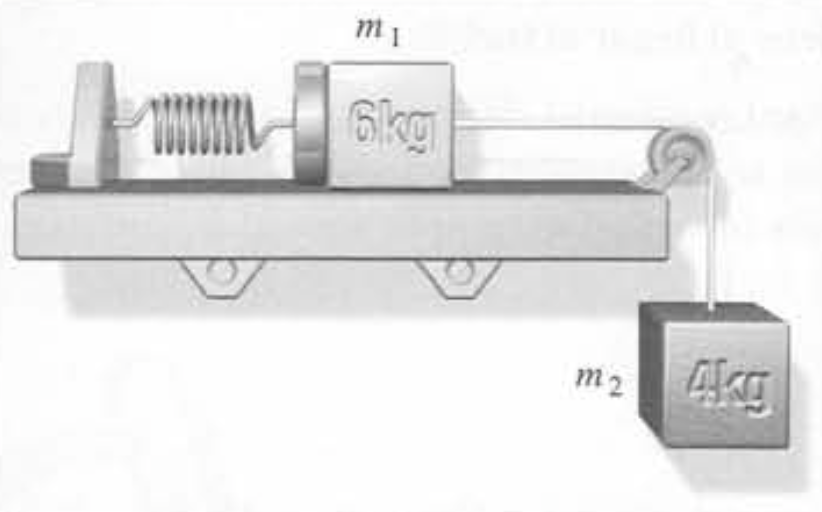
\includegraphics[width=.55\textwidth]{imagenes/imagenes04/T04IM25.png}
\end{figure}
\end{multicols}

Llamamos $\Delta x=-0.3\ \mathrm{m}$ a la compresión inicial del muelle. $h=0.4\ \mathrm{m}$ al descenso que sufre la masa $m_2$ al soltar el muelle y $\Delta s$ al desplazamiento a que se ve sometida  la masa $m_1$ al soltar el muelle. Consideramos la cuerda rígida (inelástica) por lo que ocurrirá que $\Delta s=h=0.4\ \mathrm{m}$.

Tomaremos el origen de energía potencial al nivel de la mas $m_2$ cuando el muelle está comprimido, por lo que $h$ será negativo y su energía potencial cuando haya descendido $h$ metros será $\mathcal E_p=-mgh$

Balance energético:

$\mathcal E_1=\mathcal E_{c_1}+\mathcal E_{pG_1}+\mathcal E_{pE_1}=0+0+\dfrac 1 2 k (\Delta x)^2$

$\mathcal E_1=\mathcal E_{c_1}+\mathcal E_{pG_1}+\mathcal E_{pE_1}=\dfrac 1 2 (m_1+m_2)v^2-m_2gh+0$

$\Delta \mathcal E=\dfrac 1 2 (m_1+m_2)v_2-m_2gh-\dfrac 1 2 k (\Delta x)^2$

Trabajo de la fuerza de rozamiento:

$W_{NC}=\vec F_R \cdot \overrightarrow{\Delta s}=F_R \Delta s \cos 180^o =-\mu N_1 \Delta s=-\mu m_1 g h$

 $\Delta \mathcal E=W_{NC} \to v=\sqrt{2 \dfrac{k(\Delta x)^2+(2m_2-2\mu m_1) gh}{m_1+m_2}}$
 
 Con los datos del problema, $\quad v=1.95\ \mathrm{ms}^{-1}$

\vspace{15mm} %**********************************
\begin{prob}
Se le pide diseñar un aparato para sostener a un actor de $65 \ \mathrm{kg}$ de masa que ``volará'' hacia el escenario durante la representación de una obra. Usted sujeta el arnés del actor a un saco de arena de $130 \ \mathrm{kg}$ mediante un cable de acero ligero que corre de manera uniforme en dos poleas sin fricción. Necesita $3.0 \ \mathrm{m}$ de cable entre el arnés y la polea más cercana, de modo que quede oculta detrás de una cortina. Para que el aparato funcione, el saco de arena nunca debe levantarse arriba del suelo mientras el actor se balancea desde arriba del escenario hacia el suelo. Llame $\theta$ al ángulo inicial que el cable del actor forma con la vertical. ¿Cuál es el valor máximo que tiene $\theta$ antes de que el saco de arena se levante del suelo?	
\end{prob}

\newpage %**********************************

\begin{figure}[H]
	\centering
	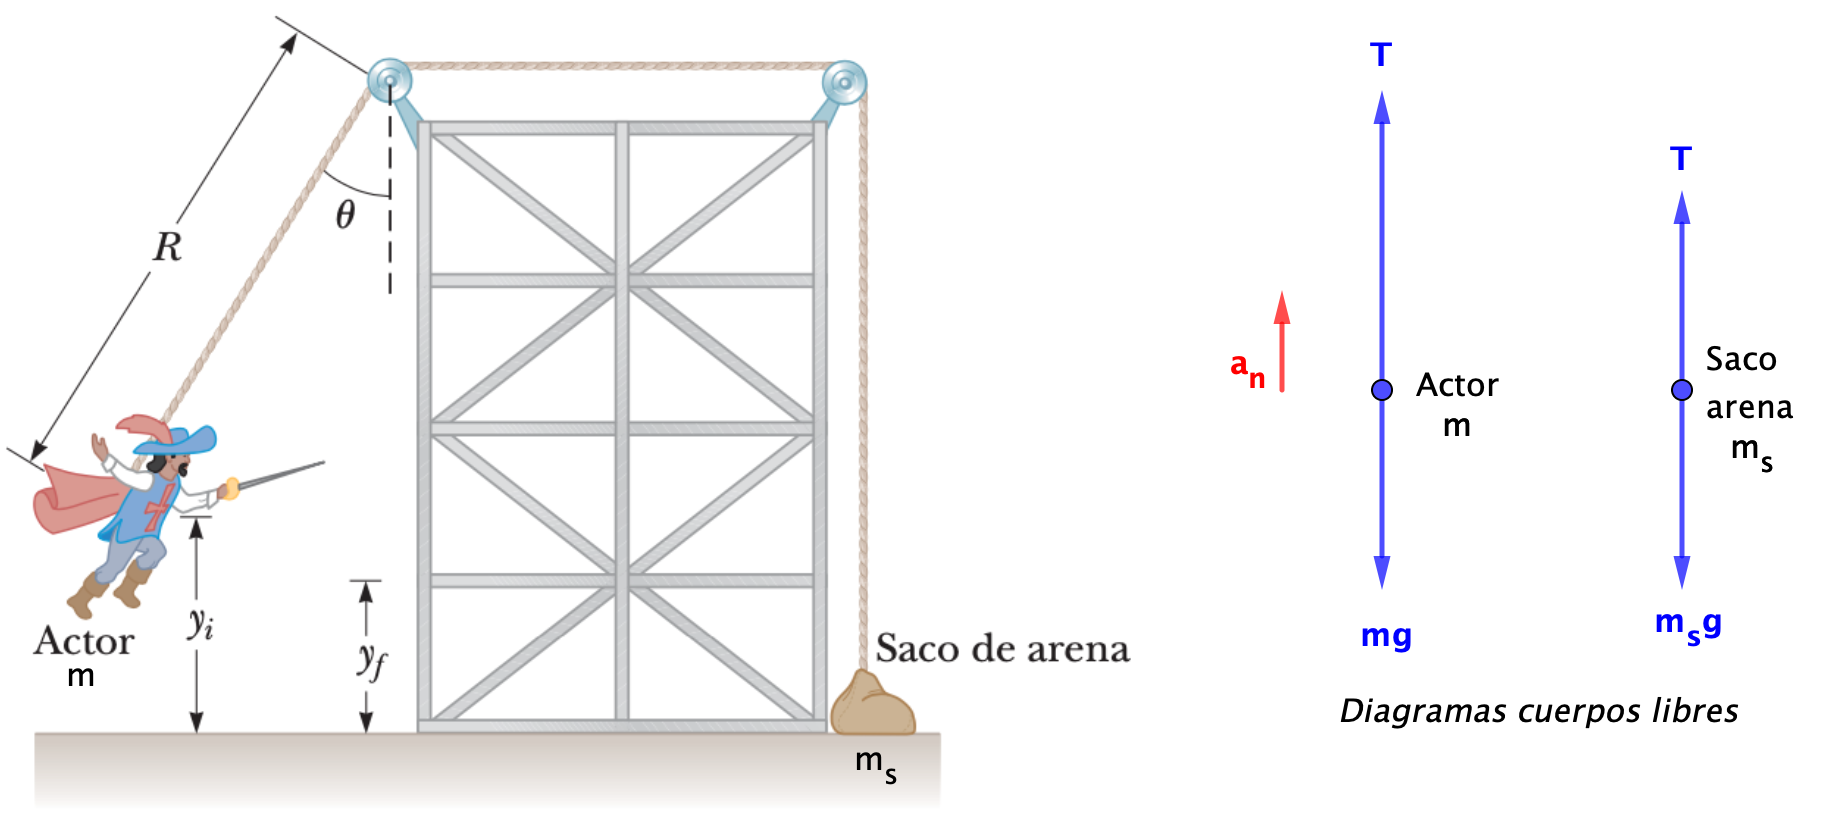
\includegraphics[width=1\textwidth]{imagenes/imagenes04/T04IM24.png}
\end{figure}

En la parte baja del movimiento circular del actor el cable es vertical y debe soportar su peso y, además, proporcionar la aceleración normal necesaria para el giro que es en dirección hacia arriba, opuesta al peso. En este punto, la tensión del cable es la más alta y es cuando el saco de arena tiene más probabilidades de levantarse del suelo, motivo por el que estableceremos ahí las consideraciones dinámicas.

En cuanto a las consideraciones energéticas, la tensión $T$ de la cuerda no realiza trabajo ya que siempre va a ser perpendicular al desplazamiento, motivo por el cual la energía se conserva. 

--- Aplicamos la conservación de la energía a los puntos $1$ cuando el actor está separado un ángulo $\theta$ respecto de la vertical y $2$ cuando baja a la posición vertical:

$\mathcal E_1=\cancelto{0}{\mathcal E_{c_1}}+\mathcal E_{p_1}=mgy_i$

$\mathcal E_2=\mathcal E_{c_2}+\mathcal E_{p_2}=\frac 1 2 m v^2+ mgy_f$

$\Delta \mathcal E=0 \to \quad v=\sqrt{2g(y_i-y_f}$

$y_f=R; \quad y_i=R\cos \theta \quad \to \qquad  v=\sqrt{2Rg(1-\cos \theta)} \ \ (1*)$

--- Dinámica de cuerpos libres a  actor y saco de arena cuando actor está en la posición vertical:

$\Sigma F_{actor}: \quad T-mg=ma_n=m\dfrac{v^2}R
\to (1*) \to \qquad T=mg(3-2\cos \theta)$


$\Sigma F_{saco}: \quad m_sg=T \to m_g=mg(3-2\cos \theta) \Rightarrow \cos \theta=\dfrac{3m-m_s}{2m}$

Con los datos del problema, $\theta=60^o$.


\begin{prob}

Queremos subir una caja de $12 \ \mathrm{kg}$ a un camión deslizándola por una rampa de $2.5 \ \mathrm{m}$ inclinada $30^o$. Un obrero, sin considerar la fricción, calcula que puede subir la caja por la rampa dándole una rapidez inicial de $5.0 \ \mathrm{ms}^{-1}$ con un empujón en la base. Sin embargo, la fricción no es despreciable; la caja sube $1.6 \ \mathrm{m}$ por la rampa, se para y se desliza de regreso. a) Suponiendo que la fuerza de fricción que actúa sobre la caja es constante, calcule su magnitud. b) ?`Qué rapidez tiene la caja al volver a la base de la rampa? c) ?`Qué velocidad debería darle el obrero a la caja si desea que suba al camión?
	
\end{prob}

\begin{figure}[H]
	\centering
	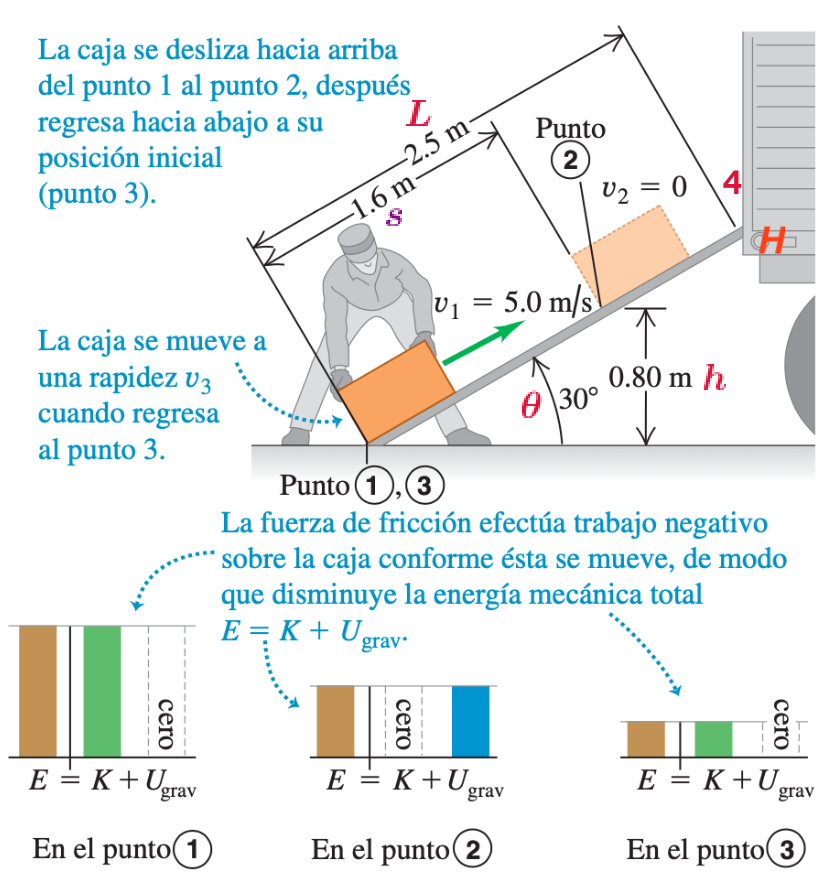
\includegraphics[width=.85\textwidth]{imagenes/imagenes04/T04IM17.png}
\end{figure}
	
$m=12\ {kg}; \ v_0=5 \ {ms}^{-1}; \; L=2.5\ {m};\; \theta=30^o;\; s=1.6\ {m};\; h=s \sin \theta;\; H=L\sin \theta$

\vspace{7mm} %**********************************
--- Balance energético puntos 1 y 2:

$\mathcal E_{c_1}=\frac 1 2 m v_o^2;\quad \mathcal E_{p_1}=0 \quad \to \quad \mathcal E_1=\frac 1 2 m v_0^2$

$\mathcal E_{c_2}=0;\quad \mathcal E_{p_2}=mgh=mgs \sin \theta \quad \to \quad \mathcal E_2=mgs \sin \theta$

$W_{NC}=-F_R  \ s \ \text{(sentido opuesto desplazamiento)}$

$\Delta \mathcal E=W_{NC} \quad \to \quad mgs \sin \theta - \frac 1 2 m v_0^2=-F_R \ s $

$F_R= \dfrac{mgs \sin \theta - \frac 1 2 m v_0^2}{s}=-35 \ \mathrm{N}$, se opone al movimiento.


\vspace{7mm} %**********************************
--- Balance energético puntos 1 y 3:

$\mathcal E_1=\frac 1 2 m v_0^2; \qquad \mathcal E_{c_3}=\frac 1 2 m v_f^2; \quad \mathcal E_{p_3}=0  \quad \to \quad \mathcal E_3=\frac 1 2 m v_f^2 $

$W_{NC}=-F_R\ (2s)$

$\Delta \mathcal E=W_{NC} \quad \to \quad \frac 1 2 m v_f^2-\frac 1 2 m v_0^2=-2F_R \ s$

$v_f=\sqrt{\dfrac{\frac 1 2 m v_0^2-2F_R\ s}{\frac 1 2 m}}=2.5\ \mathrm{ms}^{-1}$

$v_o=5\ \mathrm{ms}^{-1} \uparrow; \quad v_f=2.5\ \mathrm{ms}^{-1} \downarrow \ $, se pierde energía por la fricción.

\vspace{7mm} %**********************************
--- Balance energético puntos 1 y 4:

Deseamos que la caja llegue justo al camión, $H=L\sin \theta; v_4=0$ y nos preguntamos con que velocidad $v_i$ abría que lanzarla en este caso. Ahora la fricción es en todo el recorrido de la caja por la rampa, $L$

$\mathcal E_1=\frac 1 2 m v_i^2; \qquad \mathcal E_{c_4}=0;\;\; \mathcal E_{p_4}=mgH=mgL\sin \theta;\;\; \mathcal E_4=mgL\sin \theta$

$W_{NC}=-F_R\ L \quad \Delta \mathcal E=W_{NC} \to mgL\sin theta -\frac 1 2 m v_i^2=-F_R\ L$

$v_i=\sqrt{\frac{mgL\sin \theta + F_R\ L}{\frac 1 2 m}}\approx 6.25 \ \mathrm{m s}^{-1}$

\vspace{15mm} %**********************************
\begin{prob}.
\begin{multicols}{2}
Una niña de masa $40\ \mathrm{kg}$ se desliza hacia abajo por un tobogán inclinado $30^o$. El coeficiente de rozamiento es $\mu=0.35$. Si la niña parte del reposo desde el punto más alto del tobogán, a una altura de $4 \ \mathrm{m} $ sobre el suelo, ?`qué velocidad llevará al llegar al suelo?
	\begin{figure}[H]
	\centering
	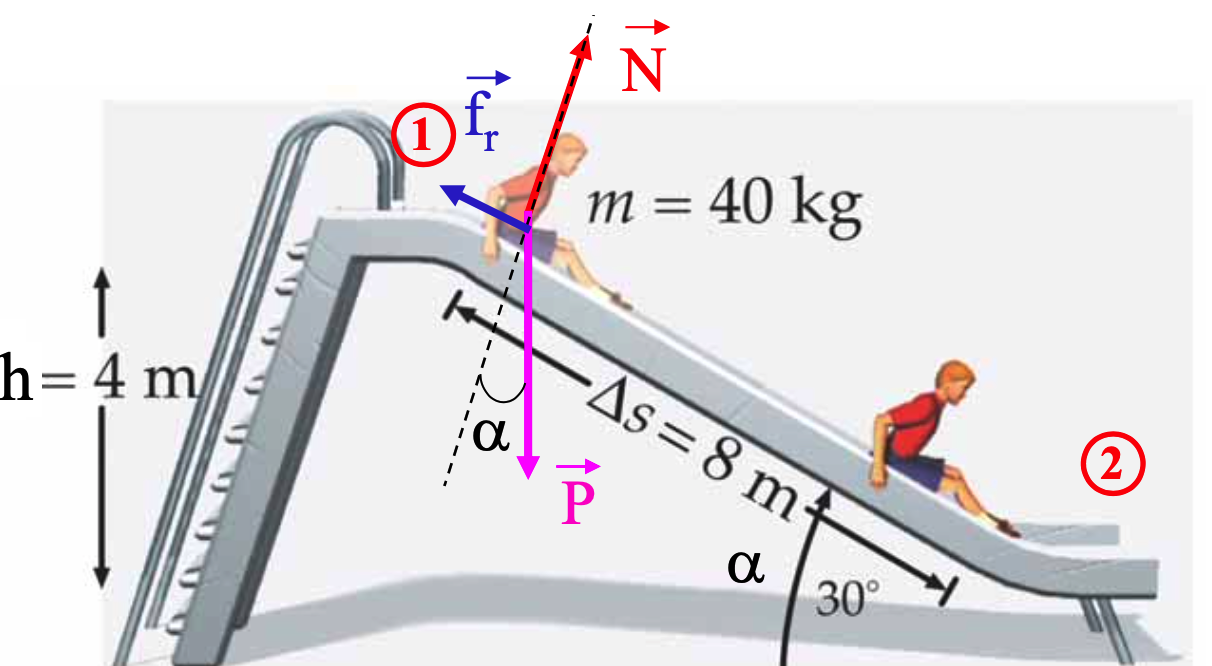
\includegraphics[width=.55\textwidth]{imagenes/imagenes04/T04IM12.png}
\end{figure}
\end{multicols}
\end{prob}

$F_R=\mu N=\mu m g \to W_{NC}=-F_R \Delta s=-\mu m g \dfrac {h}{\sin \theta}$

$\mathcal E_1=\mathcal E_{p_1}=mgh;\quad \mathcal E_2=\mathcal E_{c_2}=\frac 1 2 m v_2 \quad \to \quad \Delta \mathcal E=\frac 1 2 m v_2 - mgh$

$\Delta \mathcal E=W_{NC} \quad \to \quad \frac 1 2 m v^2-mgh=-\mu m g \dfrac {h}{\sin \theta}$

$v=\sqrt{2gh\left(1-\dfrac {\mu}{\sin \theta}  \right)}\approx 4.85\ \mathrm{ms}^{-1}$

\begin{prob}
	Una partícula de masa $m$ desliza, sin rozamiento, por una cúpula hemiesférica de radio $R$. Determinar el ángulo para el cual la partícula deja de tener contacto con la cúpula.
	
	Estudiar también el movimiento de la partícula al abandonar la cúpula hasta llegar al suelo. 
\end{prob}
\begin{multicols}{2}
--- Conservación de la energía:

$\mathcal E_1 =\mathcal E_{c_1}+\mathcal E_{p_1}=0+mgR=mgR$

$\mathcal E_2=\mathcal E_{c_2}+\mathcal E_{p_2}=\frac 1 2 m v^2+mgR\cos \theta$

$\mathcal E_1=\mathcal E_2 \to $

$v=\sqrt{2gR(1-cos \theta)}\quad (1*)$

\begin{figure}[H]
	\centering
	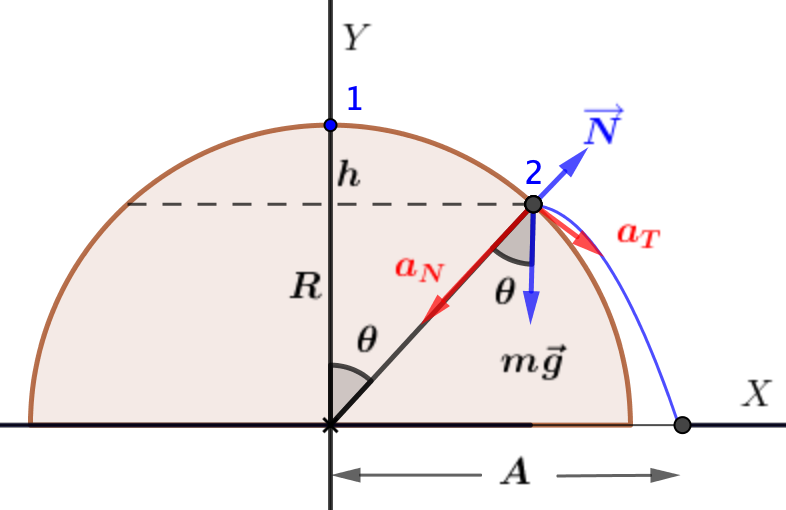
\includegraphics[width=.5\textwidth]{imagenes/imagenes04/T04IM22.png}
\end{figure}
\end{multicols}

--- Dinámica: $\begin{cases} \Sigma F_T: \quad mg\sin \theta=ma_T \\ \Sigma F_N:\quad mg\cos \theta-N=ma_N=m\dfrac {v^2}R \end{cases}$

$ \quad  N=mg\cos \theta-m\dfrac {v^2}R \quad (1*) \to \quad N=mg[3\cos \theta - 2]$

La pelota abandona la esfera cuando $\ N=0\to \cos \theta =2/3 \to \ \theta =48.19^o$

--- Ecuaciones del movimiento al abandonar la esfera: MRUA, describirá una parábola.

$\left. \begin{matrix}
x_0=R\sin \theta \quad \\ y_0=R \cos \theta \quad 	
 \end{matrix} \right|
 \left. \begin{matrix}
 v_{0_x}=v_0 \cos \theta \quad \\ v_{0_y}=v_0 \sin \theta \quad 	
 \end{matrix} \right|
 \left. \begin{matrix}
 a_x=0 \ \ \\ a_y=-g	
 \end{matrix} \right.
 \to 
 \left. \begin{matrix}
 	x=R \sin \theta + v_0 \cos \theta t \quad \quad \quad \\
 	y=R \cos \theta +  v_0 \sin \theta t - \frac 1 2 g t^2 \ 
 \end{matrix} \right.$

Haciendo $y=0 \to t=t_v$, tiempo de vuelo. $t_v \to x=x(t_v)=A$ y determinamos el alcance del tiro, la distancia a la que cae la partícula al abandonar la superficie hemiesférica.

\begin{multicols}{2}
$\quad$

$\quad$

Nota: si en vez de una semiesfera se trata de una esfera, para calcular el alcance habría que hacer $y=-R$, con el mismo sistema de referencia.

\begin{figure}[H]
	\centering
	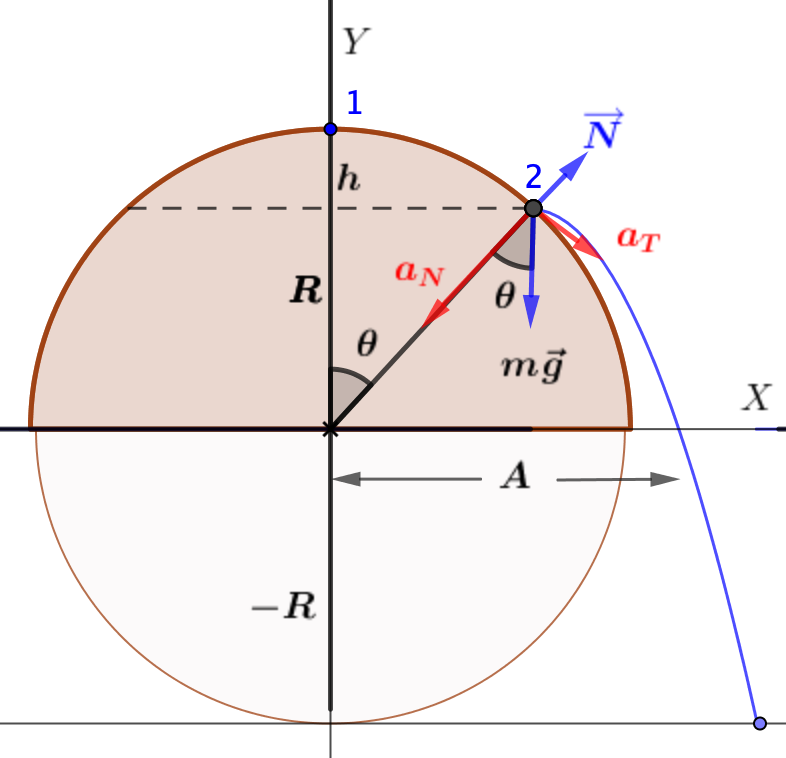
\includegraphics[width=.4\textwidth]{imagenes/imagenes04/T04IM23.png}
\end{figure}
\end{multicols}


\newpage %****************************************

\begin{myblock}{Leyes de conservación}
\begin{small}
Las leyes de conservación son las leyes físicas que postulan que durante la evolución temporal de un sistema aislado, ciertas magnitudes tienen un valor constante. Puesto que el universo entero constituye un sistema aislado, se le pueden aplicar diversas leyes de conservación.

Las leyes de conservación más importantes en física clásica son:
\begin{itemize}
\vspace{-2mm}\item Conservación del momento lineal
\vspace{-2mm} \item Conservación del momento angular
\vspace{-2mm}\item Conservación de la carga eléctrica
\vspace{-2mm}\item Conservación de la masa
\vspace{-2mm}\item Conservación de la energía
\end{itemize}

\textbf{Cantidad de movimiento}

La cantidad de movimiento, momento lineal, ímpetu o momentum es una magnitud física derivada de tipo vectorial que describe el movimiento de un cuerpo en cualquier teoría mecánica. En mecánica clásica, la cantidad de movimiento se define como el producto de la masa del cuerpo y su velocidad en un instante determinado. 

La cantidad de movimiento obedece a una ley de conservación, lo cual significa que la cantidad de movimiento total de todo sistema cerrado (o sea uno que no es afectado por fuerzas exteriores, y cuyas fuerzas internas no son disipadoras) no puede ser cambiada y permanece constante en el tiempo. 

\textbf{Conservación de la energía}

La ley de la conservación de la energía afirma que la cantidad total de energía en cualquier sistema físico aislado (sin interacción con ningún otro sistema) permanece invariable con el tiempo, aunque dicha energía puede transformarse en otra forma de energía. En resumen, la ley de la conservación de la energía afirma que la energía no se crea ni se destruye solo se transforma. En termodinámica, constituye el \emph{primer principio de la termodinámica} (la primera ley de la termodinámica).


\textbf{Momento angular}

El momento angular o momento cinético es una magnitud física, equivalente rotacional del momento lineal y representa la cantidad de movimiento de rotación de un objeto. Es una cantidad vectorial que caracteriza las propiedades de inercia de un cuerpo, que gira en relación con cierto punto. Esta magnitud desempeña respecto a las rotaciones un papel análogo al momento lineal en las traslaciones.

El nombre tradicional en español es momento cinético, pero por influencia del inglés \emph{angular momentum} hoy son frecuentes momento angular y otras variantes como cantidad de movimiento angular o ímpetu angular.

Bajo ciertas condiciones de simetría rotacional de los sistemas es una magnitud física que se mantiene constante con el tiempo a medida que el sistema va cambiando, lo cual da lugar a la llamada ley de conservación del momento angular. El momento angular para un cuerpo rígido que rota respecto a un eje es la resistencia que ofrece dicho cuerpo a la variación de la velocidad angular. Sin embargo, eso no implica que sea una magnitud exclusiva de las rotaciones; por ejemplo, el momento angular de una partícula que se mueve libremente con velocidad constante (en módulo y dirección) también se conserva.
\end{small}	
\end{myblock}



	